\section{Lists}
%\textit{Child and Configuration lists and their adapters\\
%Lister generelt, hvad er Android filosofien bag lister}
In Android the philosophy behind lists is that the majority of all applications at some point will have to implement a list object.
Therefore does Android ship with a build in list view, that supports a variety of list.
This build in list view can be modified to match any list, that the developer wishes to create, as shown in \ref{fig:listview_example}.

\begin{figure}[H]
	\centering
		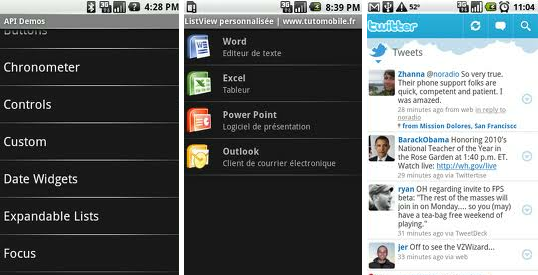
\includegraphics[width=\textwidth]{Images/Implementation/listview_example.png}
	\caption{Examples of how ListViews can be modified.}
	\label{fig:listview_example}
\end{figure}

\subsection{Benefits and Limitations}
%\textit{ Hvad er fordelen ved at bruge lister frem for at lave sin egen liste af textviews\\
%ADAPTERS\\
%Hvor langt tilbage er lister understøttet\\}
The advantage of a list view is, that we can modify the list to whatever we want it to look like without having to create any complicated programming to make it look good.
This is done by making an adapter with the layout that the items of the list is going to look like.

\begin{figure}[H]
	\centering
		\begin{verbatim}
		View v = list_item_view;
				if (v == null) {
					LayoutInflater li = (LayoutInflater) getContext().getSystemService(
							Context.LAYOUT_INFLATER_SERVICE);
					v = li.inflate(R.layout.profile_list, null);
				}
				// FIXME: Insert pictures from admin here
				Child c = items.get(position);
				if (c != null) {
					ImageView iv = (ImageView) v.findViewById(R.id.profilePic);
					TextView tv = (TextView) v.findViewById(R.id.profileName);

					if (iv != null) {
						iv.setImageResource(R.drawable.default_profile);
					}
					if (tv != null) {
						if (c.name == "Last Used") {
							tv.setText(R.string.last_used);
						} else if (c.name == "Predefined Profiles") {
							tv.setText(R.string.predefined);
						} else {
							tv.setText(c.name);
						}
					}
				}
		\end{verbatim}
	\caption{Example of an adapter to a list view}%
	\label{code:listview_adapter_example}%
\end{figure}



\subsection{Lists in WOMBAT}
%\textit{ Hvordan bruger vi lister\\
%Child listen, SubProfile listen\\
%Hvordan har det indflydelse på applikationen\\}